% =====================================================================
% ejercicio09.tex
% Responsabilidad única: ajustar la cuadrícula de árboles de clasificación, elegir árbol y umbral
% con validación, comparar con la logística e interpretar reglas e
% importancias.
% Las cifras provienen de generado/resultados.tex y generado/tabla_*.tex.
% =====================================================================
\subsection{Ejercicio 9: Caso B, árbol de clasificación e interpretación}

\paragraph{Qué buscamos.} Para el mismo problema del cáncer de mama
probamos ahora un árbol de clasificación, el modelo del Ejercicio~5a: hace
preguntas sobre las variables y cada hoja da como probabilidad de maligno
la proporción de malignos que cayeron en ella. Su atractivo es que se puede
leer como un conjunto de reglas. Elegimos el árbol y su umbral con
validación, lo comparamos con la regresión logística del Ejercicio~8 y
miramos qué variables usa.

\begin{enumerate}

\item \textbf{Cuadrícula de \texttt{DecisionTreeClassifier}.}
Ajustamos doce árboles, todas las combinaciones de
\texttt{max\_depth} $\in\{2,3,5,\texttt{None}\}$ (\texttt{None} significa sin
límite de profundidad) y \texttt{min\_samples\_leaf} $\in\{1,5,15\}$, con el
criterio de Gini del Ejercicio~5a para elegir las preguntas y
\texttt{random\_state=42} para que los resultados se puedan repetir.
Usamos los predictores originales sin estandarizar, porque a un árbol solo
le importa si un valor está por encima o por debajo de un corte, no su
escala. Recorrimos la cuadrícula con \texttt{max\_depth} por fuera y
\texttt{min\_samples\_leaf} por dentro, y ese orden quedó como último
criterio de desempate.

Nos dimos cuenta de que \texttt{min\_samples\_leaf} limita por sí solo la
profundidad: con hojas de al menos 5 o 15 muestras, los árboles con
\texttt{max\_depth} igual a 5 y a \texttt{None} resultaron idénticos
(Tabla~\ref{tab:ex9-arboles}), porque antes de llegar a profundidad 5 ya no
quedan grupos lo bastante grandes para partir. En el otro extremo, el árbol
sin ninguna restricción alcanzó ROC-AUC y F1 de entrenamiento de
$\ArbolLibreAUCTr$, es decir, clasificó perfecto el entrenamiento: señal de
que lo memorizó.

\item \textbf{Selección del árbol.}
Como en el Ejercicio~8, elegimos con el ROC-AUC de validación porque no
depende del umbral. El F1 de la tabla usa la regla
$\hat y=\mathbf{1}[p\ge0.5]$, que se lee \emph{predecir $1$ si $p\ge0.5$ y
$0$ si no}.

\begin{table}[H]
\centering
\resizebox{\textwidth}{!}{% Archivo generado automáticamente por el notebook (no editar a mano).
\begin{tabular}{lrrrrrrr}
\toprule
max\_depth & min\_samples\_leaf & ROC-AUC ent. & ROC-AUC val. & F1 ent. & F1 val. & Prof. real & Hojas \\
\midrule
2 & 1 & 0.9726 & 0.9492 & 0.9308 & 0.8571 & 2 & 4 \\
2 & 5 & 0.9726 & 0.9492 & 0.9308 & 0.8571 & 2 & 4 \\
2 & 15 & 0.9754 & 0.9656 & 0.9213 & 0.8817 & 2 & 4 \\
3 & 1 & 0.9893 & 0.8898 & 0.9762 & 0.8941 & 3 & 8 \\
3 & 5 & 0.9928 & 0.9589 & 0.9600 & 0.8941 & 3 & 7 \\
3 & 15 & 0.9854 & 0.9745 & 0.9213 & 0.8817 & 3 & 5 \\
5 & 1 & 0.9999 & 0.9270 & 0.9960 & 0.9091 & 5 & 16 \\
5 & 5 & 0.9976 & 0.9466 & 0.9647 & 0.8864 & 4 & 10 \\
5 & 15 & 0.9886 & 0.9735 & 0.9213 & 0.8817 & 4 & 6 \\
None & 1 & 1.0000 & 0.9042 & 1.0000 & 0.8764 & 6 & 17 \\
None & 5 & 0.9976 & 0.9466 & 0.9647 & 0.8864 & 4 & 10 \\
None & 15 & 0.9886 & 0.9735 & 0.9213 & 0.8817 & 4 & 6 \\
\bottomrule
\end{tabular}
}
\caption{Árboles de clasificación: ROC-AUC y F1 ($\hat y = \mathbf{1}[p\ge 0.5]$) en entrenamiento y validación.}
\label{tab:ex9-arboles}
\end{table}

Seleccionamos el árbol de \texttt{max\_depth} $=\ArbolClfMaxDepth$ y
\texttt{min\_samples\_leaf} $=\ArbolClfMinLeaf$, que tuvo el mayor ROC-AUC
de validación ($\ArbolClfAUCVal$), con profundidad real $\ArbolClfProf$ y
$\ArbolClfHojas$ hojas. Su máximo es único (una sola fila lo alcanza), así
que esta vez no hubo que desempatar. Los árboles con hojas de una sola
muestra y profundidad real de 3 o más quedaron entre los peores en
validación pese a tener los mejores valores de entrenamiento, el mismo
patrón de sobreajuste del Ejercicio~7.

\item \textbf{Umbral del árbol y candidato final de clasificación.}
Repetimos el procedimiento del Ejercicio~8c con los mismos siete umbrales
y las mismas reglas (menor costo, luego mayor recall, luego menor umbral).

\begin{table}[H]
\centering
\small
% Archivo generado automáticamente por el notebook (no editar a mano).
\begin{tabular}{lrrrrrr}
\toprule
Umbral & Precisión & Recall & F1 & FP & FN & Costo L \\
\midrule
0.2 & 0.7636 & 0.9767 & 0.8571 & 13 & 1 & 18 \\
0.3 & 0.8200 & 0.9535 & 0.8817 & 9 & 2 & 19 \\
0.4 & 0.8200 & 0.9535 & 0.8817 & 9 & 2 & 19 \\
0.5 & 0.8200 & 0.9535 & 0.8817 & 9 & 2 & 19 \\
0.6 & 0.9487 & 0.8605 & 0.9024 & 2 & 6 & 32 \\
0.7 & 1.0000 & 0.7907 & 0.8831 & 0 & 9 & 45 \\
0.8 & 1.0000 & 0.7907 & 0.8831 & 0 & 9 & 45 \\
\bottomrule
\end{tabular}

\caption{Umbrales para el árbol seleccionado (validación).}
\label{tab:ex9-umbrales}
\end{table}

Al ver la Tabla~\ref{tab:ex9-umbrales} nos llamó la atención que varias
filas coincidieran, y la razón es la del Ejercicio~5b: el árbol solo puede
dar tantas probabilidades distintas como hojas tiene (la proporción de
malignos de cada hoja), así que todos los umbrales que caen entre dos de
esos valores producen exactamente las mismas predicciones. El menor costo
lo obtuvimos con $\boldsymbol{t=\ArbolT}$ ($L=\ArbolCostoSel$, con
$FP=\ArbolFPSel$ y $FN=\ArbolFNSel$), donde la regla $p\ge t$ incluye la hoja
cuya proporción de malignos es exactamente 0.2.

Para elegir el candidato final de clasificación entre la logística y el
árbol comparamos sus costos de validación (en empate habríamos mirado el
ROC-AUC). El costo del árbol es claramente mayor que el de la regresión
logística ($L=\LogitCostoSel$), por lo que nos quedamos con la
\textbf{regresión logística con $C=\LogitC$ y $t=\LogitT$}, sin necesidad de
desempates; su ROC-AUC de validación también es mayor ($\LogitAUCVal$
frente a $\ArbolClfAUCVal$).

\paragraph{Puente con el Ejercicio~3d: umbral teórico y calibración.}
En el Ejercicio~3d demostramos que, si las probabilidades están bien
calibradas, el umbral de costo mínimo es $t^*=c_{FP}/(c_{FP}+c_{FN})$, que
para $L=FP+5FN$ (es decir, $c_{FP}=1$ y $c_{FN}=5$) vale
$t^*=1/6\approx\TTeorico$. Nos pareció que valía la pena contrastar esa
predicción de la teoría con lo que elegimos en la práctica
(Tabla~\ref{tab:ex9-puente} y Figura~\ref{fig:ex9-calibracion}). El
contraste es solo descriptivo: el enunciado fija la rejilla de siete
umbrales, así que $t^*$ no lo usamos para seleccionar ni cambia ningún
candidato.

Para revisar la calibración usamos dos herramientas. La \emph{curva de
calibración} ordena las muestras de validación por su probabilidad
predicha, las reparte en cinco grupos de igual tamaño y, para cada grupo,
compara la probabilidad predicha promedio con la fracción de malignos que
de verdad hay en él; si el modelo está bien calibrado, los puntos caen
sobre la diagonal. El \emph{puntaje de Brier} (Tabla~\ref{tab:metricas})
resume en un número qué tan cerca están las probabilidades de lo que
ocurrió.

\begin{table}[H]
\centering
\small
% Archivo generado automáticamente por el notebook (no editar a mano).
\begin{tabular}{lrlrrrr}
\toprule
Modelo & Brier & t elegido & L (t elegido) & L (t* = 1/6) & FP (t*) & FN (t*) \\
\midrule
Regresión logística & 0.0201 & 0.7 & 5 & 15 & 10 & 1 \\
Árbol & 0.0528 & 0.2 & 18 & 18 & 13 & 1 \\
\bottomrule
\end{tabular}

\caption{Umbral teórico $t^*=1/6$ del Ejercicio~3d frente al umbral
elegido, y puntaje de Brier (validación).}
\label{tab:ex9-puente}
\end{table}

\begin{figure}[H]
    \centering
    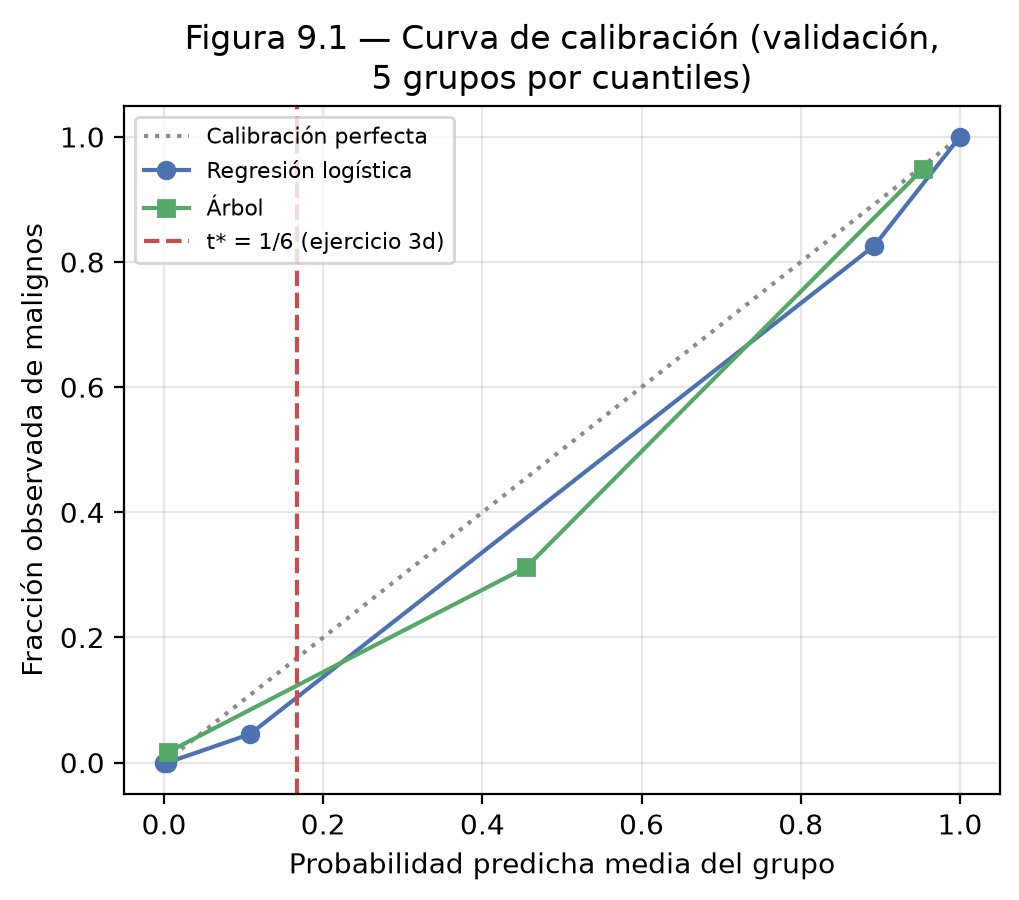
\includegraphics[width=0.6\textwidth]{figuras/ex9_calibracion.png}
    \caption{Curva de calibración en validación (cinco grupos por
    cuantiles): fracción observada de malignos frente a la probabilidad
    predicha media de cada grupo, con $t^*=1/6$ marcado en rojo.}
    \label{fig:ex9-calibracion}
\end{figure}

En el árbol la teoría y la práctica coincidieron, pues $t^*$ produce
exactamente las mismas predicciones que $t=\ArbolT$ ($L=\ArbolCostoTeo$):
ninguna hoja tiene una probabilidad entre $\TTeorico$ y $0.2$, y $0.2$ es
el valor de la rejilla más cercano a $t^*$. En la regresión logística, en
cambio, $t^*$ daría $L=\LogitCostoTeo$ ($FP=\LogitFPTeo$, $FN=\LogitFNTeo$),
el triple que el umbral elegido, y le dimos varias vueltas hasta ver que
la diferencia se explica por las condiciones que exige el resultado
teórico:
\begin{itemize}
    \item \textbf{La calibración no es perfecta.} En el grupo de
    probabilidades bajas (probabilidad predicha media de $\LogitCalMedia$)
    la fracción real de malignos es solo $\LogitCalFrac$. O sea, en esa
    zona el modelo exagera el riesgo, justo donde cae $t^*$, y bajar el
    umbral hasta allí agrega falsos positivos que en realidad son
    benignos.
    \item \textbf{Un caso puntual de esta validación.} El único maligno no
    detectado tiene $p=\LogitPMalMin$, por debajo incluso de $t^*$, así que
    ningún umbral de la rejilla lo recupera y bajar el umbral solo cuesta
    falsos positivos.
    \item \textbf{Las probabilidades de la logística son mejores, pero con
    pocos datos.} El puntaje de Brier ($\LogitBrier$ frente a
    $\ArbolBrier$) confirma que la logística da probabilidades más
    cercanas a la realidad que el árbol, aunque con $\NClfVal$ muestras
    cada punto de la curva de calibración se calcula con apenas una
    quinta parte de ellas y tiene bastante error de muestreo.
\end{itemize}
Lo que sacamos en limpio es que $t^*$ es una referencia teórica valiosa
cuyo supuesto clave (la calibración) hay que verificar antes de aplicarla,
y que el umbral alto de la logística descansa en muy pocos casos,
advertencia que retomamos al evaluar en prueba (Ejercicio~10b).

\item \textbf{Visualización y regla de una hoja.}
El árbol seleccionado tiene profundidad real $\ArbolClfProf$, de modo que la
Figura~\ref{fig:ex9-arbol}, limitada a tres niveles, lo muestra completo y
no está recortada. Cada recuadro es un nodo y muestra, de arriba abajo,
la pregunta que hace (si la respuesta es sí, la muestra baja por la
izquierda), su impureza de Gini, cuántas muestras de entrenamiento llegan
a él, cuántas son \emph{[benignas, malignas]} y la clase que predeciría;
el color va de naranja (mayoría benigna) a azul (mayoría maligna), más
intenso entre más puro es el nodo. La raíz pregunta por \texttt{worst perimeter} (el perímetro de los
núcleos más grandes) y el segundo nivel, en ambas ramas, por
\texttt{worst concave points} (cuántos hundimientos tienen los núcleos con
más hundimientos). Escrita como regla, la ruta hasta la hoja con más
muestras malignas es la siguiente, y esa hoja contiene $\HojaEjMuestras$
muestras de entrenamiento con proporción de malignos $\HojaEjProp$:
% Archivo generado automáticamente por el notebook (no editar a mano).
\begin{verbatim}
if worst perimeter > 112.8000:
    if worst concave points > 0.1396:
        predecir maligno  # p = 1.0000
\end{verbatim}

\noindent En palabras: si los núcleos más grandes tienen un perímetro
mayor que el corte y además muchos hundimientos en el borde, el árbol
declara la muestra maligna.

\begin{figure}[H]
    \centering
    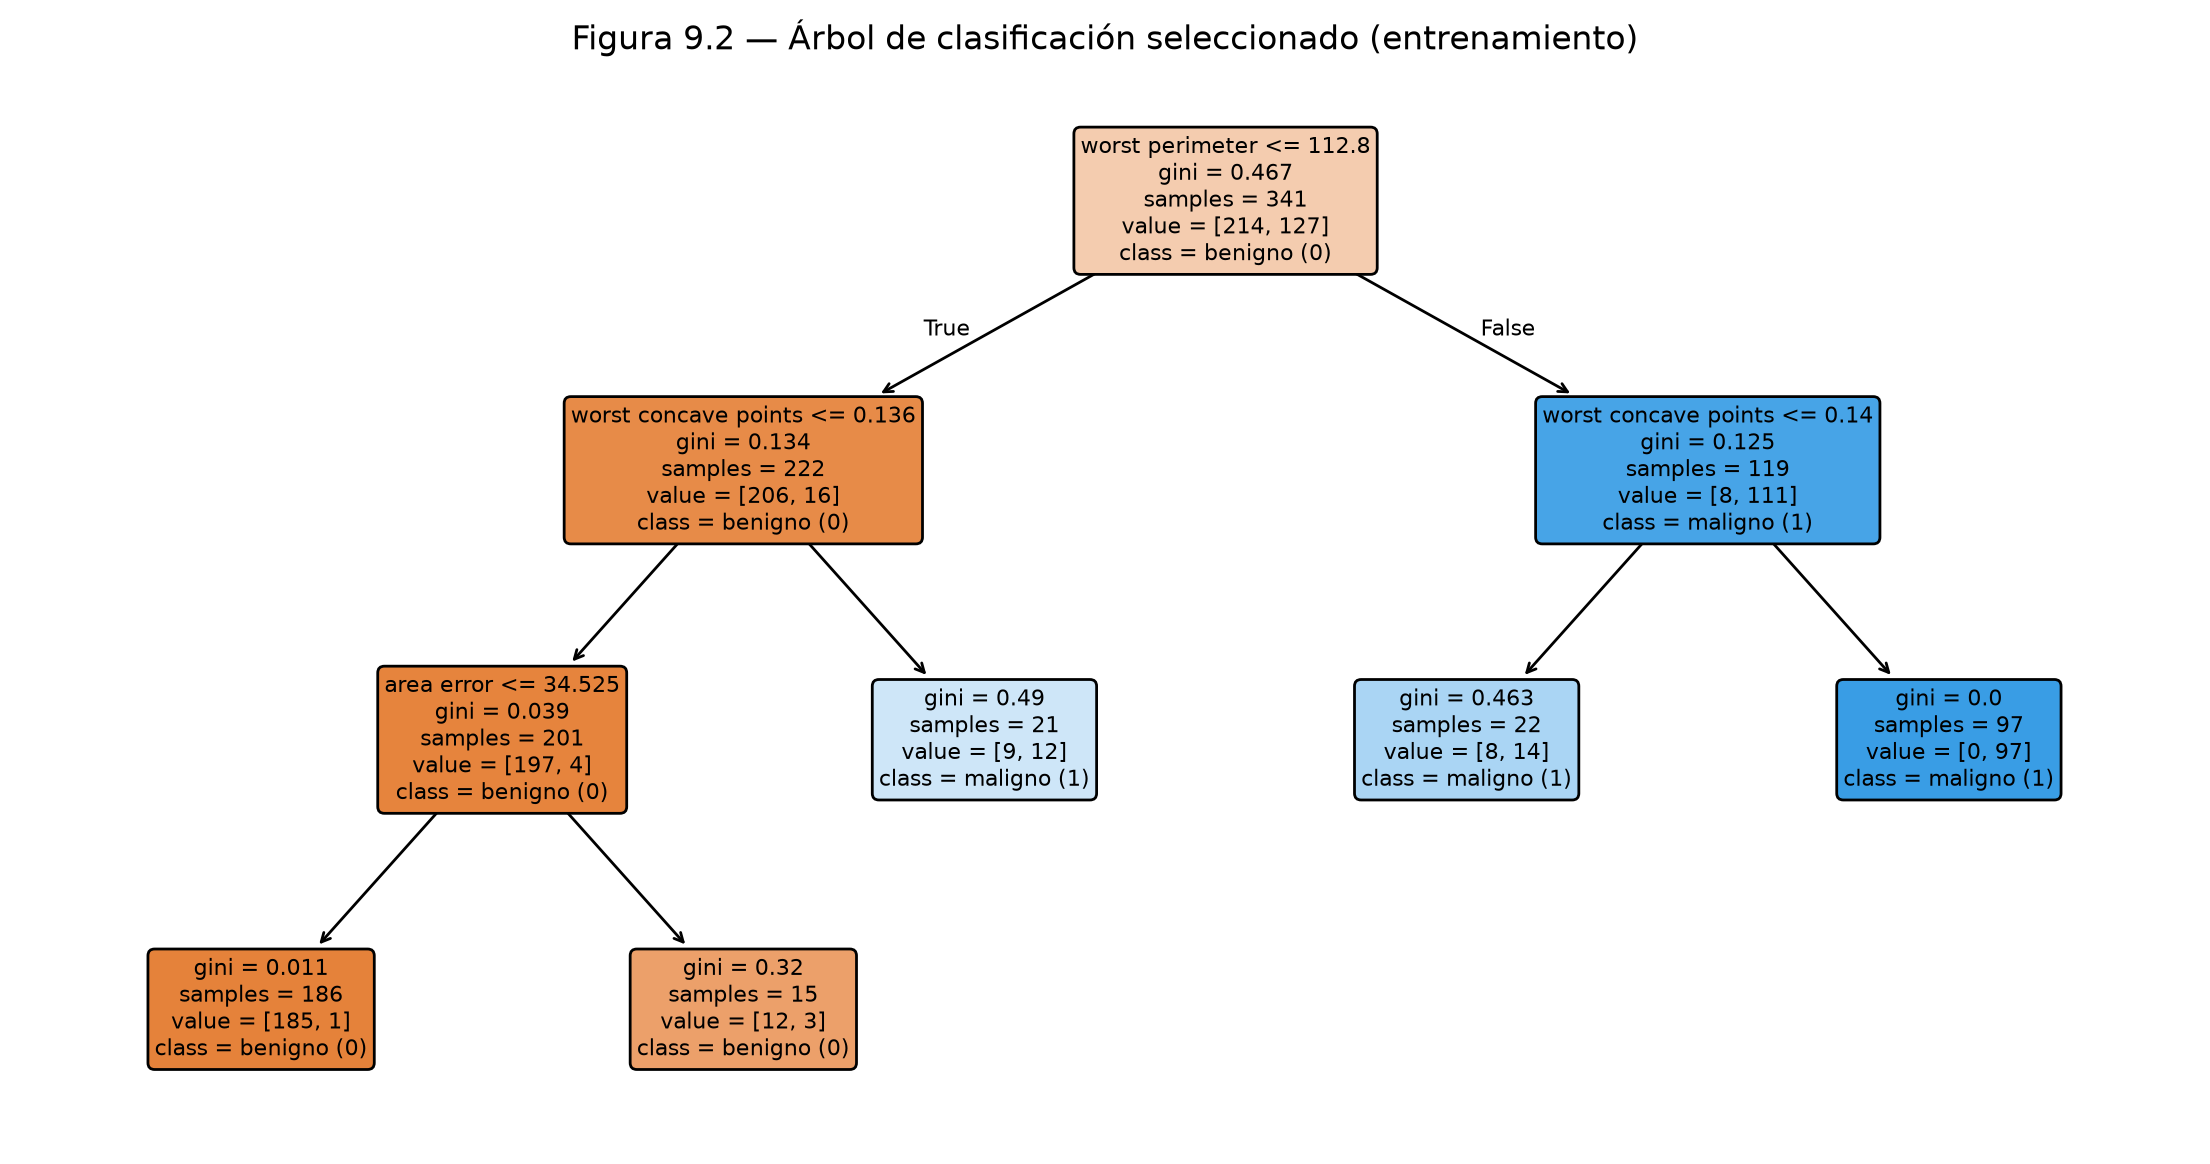
\includegraphics[width=\textwidth]{figuras/ex9_arbol.png}
    \caption{Árbol de clasificación seleccionado, ajustado con entrenamiento (conteos por clase en cada nodo).}
    \label{fig:ex9-arbol}
\end{figure}

\item \textbf{Importancias, coeficientes y sobreajuste.}
La \emph{importancia} de una variable en un árbol es cuánta impureza de
Gini (Ejercicio~5a) se redujo en total gracias a las preguntas sobre esa
variable, normalizada para que todas sumen 1. El árbol concentra casi
toda la importancia en \texttt{worst perimeter} ($\ImpPerimetro$) y
\texttt{worst concave points} ($\ImpPuntos$), con un aporte marginal de
\texttt{area error} ($\ImpAreaError$), y solo $\ImpNoNulas$ de los 30
predictores tienen importancia distinta de cero
(Figura~\ref{fig:ex9-imp} y Tabla~\ref{tab:ex9-imp}). La regresión
logística, en cambio, reparte el peso entre muchas variables, y nos
sorprendió que \texttt{worst perimeter} ocupe apenas el puesto
$\RangoPerimetro$ por tamaño de coeficiente y \texttt{worst concave
points} el $\RangoPuntos$.

Sin embargo, las dos cosas no se pueden comparar directamente. La
importancia nunca es negativa ni tiene signo (no dice si la variable sube o
baja el riesgo), y depende de qué variable eligió primero el árbol entre
varias casi intercambiables: perímetro, radio y área miden casi lo mismo,
así que si el árbol usa una, las otras ya no aportan y quedan en cero. El
coeficiente logístico, por su parte, es un cambio en log-odds por
desviación estándar, con signo y condicional a las demás variables. Ninguno
de los dos implica efectos causales.

\begin{figure}[H]
    \centering
    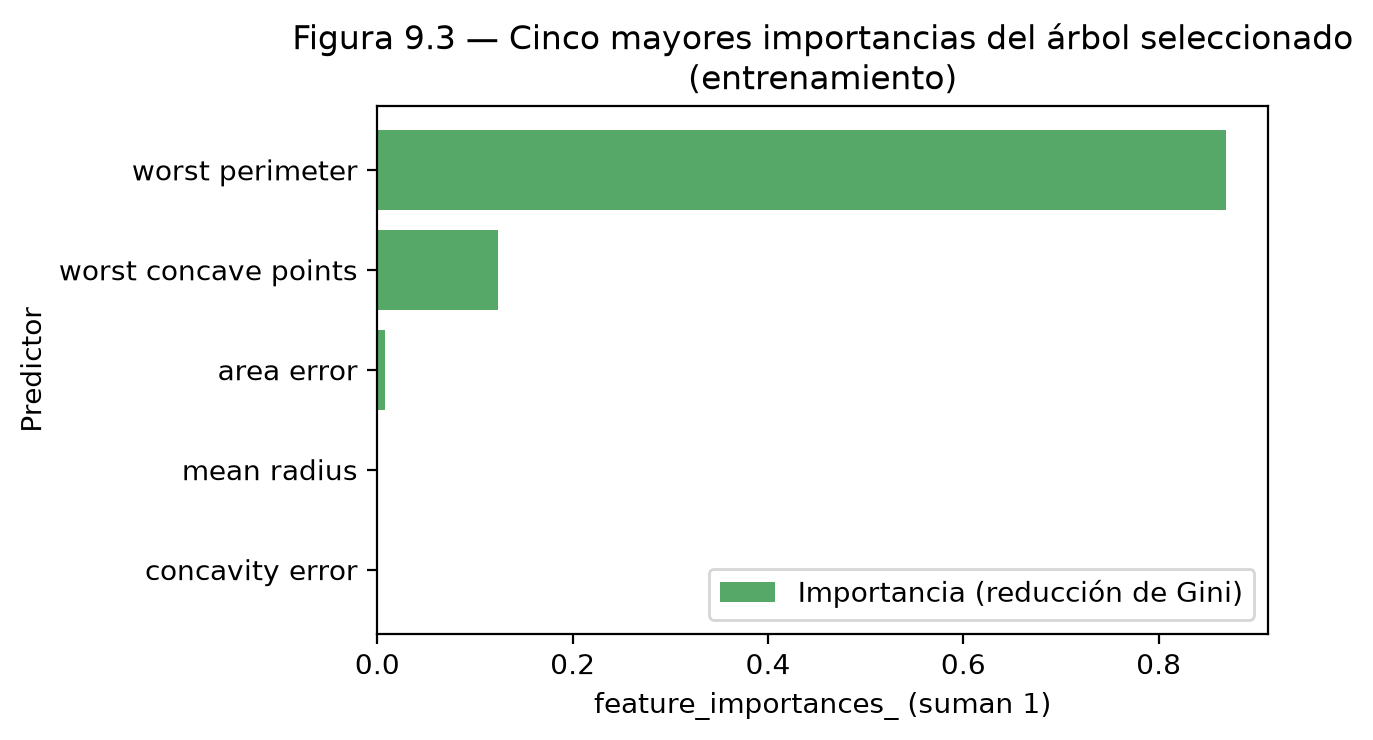
\includegraphics[width=0.66\textwidth]{figuras/ex9_importancias.png}
    \caption{Cinco mayores importancias del árbol seleccionado (entrenamiento).}
    \label{fig:ex9-imp}
\end{figure}

\begin{table}[H]
\centering
\small
% Archivo generado automáticamente por el notebook (no editar a mano).
\begin{tabular}{lrrr}
\toprule
Predictor & Importancia árbol & Coef. logística & Rango $|\beta|$ logística \\
\midrule
worst perimeter & 0.8686 & 0.6617 & 11 \\
worst concave points & 0.1234 & 0.5368 & 15 \\
area error & 0.0080 & 0.7822 & 7 \\
mean radius & 0.0000 & 0.4942 & 18 \\
concavity error & 0.0000 & $-$0.0964 & 28 \\
\bottomrule
\end{tabular}

\caption{Importancias del árbol frente a coeficientes estandarizados de la logística.}
\label{tab:ex9-imp}
\end{table}

En cuanto al sobreajuste, la Tabla~\ref{tab:ex9-arboles} muestra evidencia
clara en los árboles con \texttt{min\_samples\_leaf} $=1$, en especial el
árbol sin restricciones, que pasó de ROC-AUC $\ArbolLibreAUCTr$ y F1
$\ArbolLibreFUnoTr$ en entrenamiento a $\ArbolLibreAUCVal$ y
$\ArbolLibreFUnoVal$ en validación: perfecto con lo que ya vio, bastante
peor con lo nuevo. Los árboles con \texttt{min\_samples\_leaf} $=15$,
incluido el seleccionado (ROC-AUC de $\ArbolClfAUCTr$ en entrenamiento y
$\ArbolClfAUCVal$ en validación), fueron los que mejor trasladaron su
desempeño a validación.

\end{enumerate}
